\documentclass{article}\usepackage[]{graphicx}\usepackage[]{color}
%% maxwidth is the original width if it is less than linewidth
%% otherwise use linewidth (to make sure the graphics do not exceed the margin)
\makeatletter
\def\maxwidth{ %
  \ifdim\Gin@nat@width>\linewidth
    \linewidth
  \else
    \Gin@nat@width
  \fi
}
\makeatother

\definecolor{fgcolor}{rgb}{0.345, 0.345, 0.345}
\newcommand{\hlnum}[1]{\textcolor[rgb]{0.686,0.059,0.569}{#1}}%
\newcommand{\hlstr}[1]{\textcolor[rgb]{0.192,0.494,0.8}{#1}}%
\newcommand{\hlcom}[1]{\textcolor[rgb]{0.678,0.584,0.686}{\textit{#1}}}%
\newcommand{\hlopt}[1]{\textcolor[rgb]{0,0,0}{#1}}%
\newcommand{\hlstd}[1]{\textcolor[rgb]{0.345,0.345,0.345}{#1}}%
\newcommand{\hlkwa}[1]{\textcolor[rgb]{0.161,0.373,0.58}{\textbf{#1}}}%
\newcommand{\hlkwb}[1]{\textcolor[rgb]{0.69,0.353,0.396}{#1}}%
\newcommand{\hlkwc}[1]{\textcolor[rgb]{0.333,0.667,0.333}{#1}}%
\newcommand{\hlkwd}[1]{\textcolor[rgb]{0.737,0.353,0.396}{\textbf{#1}}}%

\usepackage{framed}
\makeatletter
\newenvironment{kframe}{%
 \def\at@end@of@kframe{}%
 \ifinner\ifhmode%
  \def\at@end@of@kframe{\end{minipage}}%
  \begin{minipage}{\columnwidth}%
 \fi\fi%
 \def\FrameCommand##1{\hskip\@totalleftmargin \hskip-\fboxsep
 \colorbox{shadecolor}{##1}\hskip-\fboxsep
     % There is no \\@totalrightmargin, so:
     \hskip-\linewidth \hskip-\@totalleftmargin \hskip\columnwidth}%
 \MakeFramed {\advance\hsize-\width
   \@totalleftmargin\z@ \linewidth\hsize
   \@setminipage}}%
 {\par\unskip\endMakeFramed%
 \at@end@of@kframe}
\makeatother

\definecolor{shadecolor}{rgb}{.97, .97, .97}
\definecolor{messagecolor}{rgb}{0, 0, 0}
\definecolor{warningcolor}{rgb}{1, 0, 1}
\definecolor{errorcolor}{rgb}{1, 0, 0}
\newenvironment{knitrout}{}{} % an empty environment to be redefined in TeX

\usepackage{alltt}
\usepackage{graphicx}
%% for inline R code: if the inline code is not correctly parsed, you will see a message
\newcommand{\rinline}[1]{SOMETHING WRONG WITH knitr}


\IfFileExists{upquote.sty}{\usepackage{upquote}}{}
\begin{document}

\section{Testing}
We implemented testing functions for each method to ensure that each 
function takes proper inputs and returns desired outputs. Each method 
functions properly when tested using small data sets. In order to test the 
functionality of our genetic algorithm, we employed a larger, more realistic 
data set. We compared the models selected using our genetic algorithim with a 
well-known model selection method, the stepwise model selection using AIC, 
implemented in R in the \texttt{stepAIC} function available in the 
\texttt{MASS} package.

This data set was obtained from surveys about how video games 
affect grades. There are 15 variables in the data set -- time (number of 
hours play), like (whether like to play), where (where to play), freq (how 
often), busy (play if busy), educ (playing educational), sex, age, home 
(computer at home), math (hate math), work (number of hours work per weeek), 
own (own PC), cdrom (PC has CD-rom), email (have Email) and grade. The 
dependent variable is grade. Completed data were obtained from 91 students 
during Fall 1994 at Berkeley. The data source can be found at the Stat Labs 
website for University of California, Berkeley. 

The following results are obtained using our genetic algorithim.

\begin{knitrout}
\definecolor{shadecolor}{rgb}{0.969, 0.969, 0.969}\color{fgcolor}\begin{kframe}
\begin{alltt}
\hlstd{data} \hlkwb{<-} \hlkwd{read.table}\hlstd{(}\hlstr{"../data/video.txt"}\hlstd{,} \hlkwc{header} \hlstd{=} \hlnum{TRUE}\hlstd{,} \hlkwc{quote} \hlstd{=} \hlstr{"\textbackslash{}""}\hlstd{)}
\hlstd{ga} \hlkwb{<-} \hlkwd{select_model}\hlstd{(data,}
                   \hlkwc{yvar} \hlstd{=} \hlstr{"grade"}\hlstd{,}
                   \hlkwc{pop_size} \hlstd{=} \hlkwd{nrow}\hlstd{(data)}\hlopt{*}\hlnum{2}\hlstd{,}
                   \hlkwc{num_max_iterations} \hlstd{=} \hlnum{50}\hlstd{,}
                   \hlkwc{model} \hlstd{=} \hlstr{"glm"}\hlstd{,}
                   \hlkwc{glm_family} \hlstd{=} \hlstr{"gaussian"}\hlstd{)}
\end{alltt}
\end{kframe}
\end{knitrout}

\begin{knitrout}
\definecolor{shadecolor}{rgb}{0.969, 0.969, 0.969}\color{fgcolor}\begin{kframe}
\begin{alltt}
\hlstd{res} \hlkwb{<-} \hlkwd{summary}\hlstd{(ga)}
\end{alltt}
\begin{verbatim}
## Model 1 :
##  grade ~ where + freq + busy + sex + home + math 
##  AIC = 157.6 
##  --------------------------------------------------
## Model 2 :
##  grade ~ freq + educ + sex + home + math 
##  AIC = 158.2 
##  --------------------------------------------------
## Model 3 :
##  grade ~ freq + busy + sex + home + math 
##  AIC = 158.3 
##  --------------------------------------------------
## Model 4 :
##  grade ~ where + freq + busy + sex + home + math + own 
##  AIC = 158.4 
##  --------------------------------------------------
## Model 5 :
##  grade ~ where + freq + busy + sex + home + math + email 
##  AIC = 158.6 
##  --------------------------------------------------
\end{verbatim}
\end{kframe}
\end{knitrout}

The following results are obtained using the \texttt{stepAIC} function.

\begin{knitrout}
\definecolor{shadecolor}{rgb}{0.969, 0.969, 0.969}\color{fgcolor}\begin{kframe}
\begin{alltt}
\hlkwd{library}\hlstd{(MASS)}
\hlstd{mod} \hlkwb{<-} \hlkwd{glm}\hlstd{(grade} \hlopt{~} \hlstd{.,} \hlkwc{data} \hlstd{= data)}
\hlstd{res_step} \hlkwb{<-} \hlkwd{stepAIC}\hlstd{(mod)}
\end{alltt}
\begin{verbatim}
## Start:  AIC=167.2
## grade ~ time + like + where + freq + busy + educ + sex + age + 
##     home + math + work + own + cdrom + email
## 
##         Df Deviance AIC
## - age    1     23.6 165
## - where  1     23.6 166
## - time   1     23.6 166
## - like   1     23.7 166
## - educ   1     23.8 166
## - cdrom  1     23.8 166
## - work   1     23.9 166
## - email  1     23.9 167
## - busy   1     23.9 167
## <none>         23.6 167
## - math   1     24.2 168
## - own    1     24.2 168
## - freq   1     24.6 169
## - home   1     25.8 174
## - sex    1     27.4 179
## 
## Step:  AIC=165.3
## grade ~ time + like + where + freq + busy + educ + sex + home + 
##     math + work + own + cdrom + email
## 
##         Df Deviance AIC
## - where  1     23.7 164
## - time   1     23.7 164
## - like   1     23.8 164
## - educ   1     23.8 164
## - cdrom  1     23.8 164
## - work   1     23.9 165
## - busy   1     24.0 165
## - email  1     24.0 165
## <none>         23.6 165
## - math   1     24.2 166
## - own    1     24.3 166
## - freq   1     24.6 167
## - home   1     25.9 172
## - sex    1     27.5 178
## 
## Step:  AIC=163.7
## grade ~ time + like + freq + busy + educ + sex + home + math + 
##     work + own + cdrom + email
## 
##         Df Deviance AIC
## - like   1     23.9 162
## - cdrom  1     23.9 162
## - busy   1     24.0 163
## - time   1     24.0 163
## - work   1     24.0 163
## - educ   1     24.1 164
## - math   1     24.2 164
## <none>         23.7 164
## - email  1     24.2 164
## - own    1     24.4 165
## - freq   1     24.8 166
## - home   1     26.1 170
## - sex    1     27.9 177
## 
## Step:  AIC=162.4
## grade ~ time + freq + busy + educ + sex + home + math + work + 
##     own + cdrom + email
## 
##         Df Deviance AIC
## - cdrom  1     24.1 161
## - time   1     24.2 162
## - work   1     24.2 162
## - busy   1     24.2 162
## - math   1     24.3 162
## - email  1     24.4 162
## - educ   1     24.4 162
## <none>         23.9 162
## - own    1     24.6 163
## - freq   1     25.0 164
## - home   1     26.2 169
## - sex    1     27.9 175
## 
## Step:  AIC=161.2
## grade ~ time + freq + busy + educ + sex + home + math + work + 
##     own + email
## 
##         Df Deviance AIC
## - time   1     24.4 160
## - work   1     24.4 160
## - busy   1     24.5 161
## - math   1     24.5 161
## - educ   1     24.6 161
## <none>         24.1 161
## - email  1     24.6 161
## - own    1     24.7 162
## - freq   1     25.1 163
## - home   1     26.6 168
## - sex    1     28.6 175
## 
## Step:  AIC=160.3
## grade ~ freq + busy + educ + sex + home + math + work + own + 
##     email
## 
##         Df Deviance AIC
## - work   1     24.7 160
## - busy   1     24.8 160
## - email  1     24.8 160
## - educ   1     24.9 160
## - math   1     24.9 160
## <none>         24.4 160
## - own    1     25.0 161
## - freq   1     25.6 163
## - home   1     27.1 168
## - sex    1     28.7 173
## 
## Step:  AIC=159.6
## grade ~ freq + busy + educ + sex + home + math + own + email
## 
##         Df Deviance AIC
## - email  1     25.1 159
## - busy   1     25.2 159
## - own    1     25.2 159
## - educ   1     25.2 159
## <none>         24.7 160
## - math   1     25.8 162
## - freq   1     25.9 162
## - home   1     27.3 167
## - sex    1     28.8 171
## 
## Step:  AIC=159.2
## grade ~ freq + busy + educ + sex + home + math + own
## 
##        Df Deviance AIC
## - own   1     25.5 159
## - educ  1     25.6 159
## - busy  1     25.6 159
## <none>        25.1 159
## - math  1     26.2 161
## - freq  1     26.3 161
## - home  1     27.8 166
## - sex   1     29.2 171
## 
## Step:  AIC=158.6
## grade ~ freq + busy + educ + sex + home + math
## 
##        Df Deviance AIC
## - busy  1     26.0 158
## - educ  1     26.0 158
## <none>        25.5 159
## - math  1     26.6 160
## - freq  1     26.7 161
## - home  1     27.8 164
## - sex   1     29.4 169
## 
## Step:  AIC=158.2
## grade ~ freq + educ + sex + home + math
## 
##        Df Deviance AIC
## <none>        26.0 158
## - freq  1     26.7 159
## - math  1     26.8 159
## - educ  1     27.4 161
## - home  1     28.4 164
## - sex   1     29.8 168
\end{verbatim}
\end{kframe}
\end{knitrout}

The best model found using genetic algorithim was: y $\sim$
where + freq + busy + sex + home + math, 
with an AIC of 157.56. This result 
is better than that of 158.23 that
we obtained using the \texttt{stepAIC} function. 

Finally, we plotted the best AIC for each generation to see how the best AIC 
has changed over generations. 

\begin{knitrout}
\definecolor{shadecolor}{rgb}{0.969, 0.969, 0.969}\color{fgcolor}\begin{kframe}
\begin{alltt}
\hlkwd{par}\hlstd{(}\hlkwc{cex} \hlstd{=} \hlnum{0.8}\hlstd{)}
\hlkwd{plot}\hlstd{(ga)}
\end{alltt}
\end{kframe}
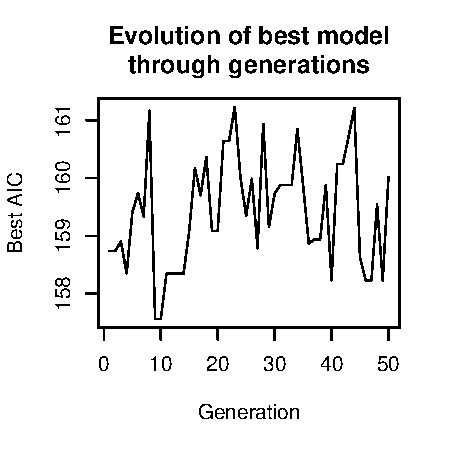
\includegraphics[width=\maxwidth]{figure/latex-unnamed-chunk-4} 

\end{knitrout}

From the plot, we can see that the best model was found at generation 9. 

\end{document}
